\documentclass[10pt,landscape]{article}

\usepackage[margin=0.5in,twocolumn]{geometry}
\usepackage{amsmath}
\usepackage{graphicx}

\setlength{\parindent}{0pt}

\title{ICPC Math Table}
\date{}

\begin{document}

\maketitle

* $p$ is prime

\section{Number Theory}

\fbox{\textbf{Fermat's little theorem}}
\begin{align*}
	a^{p-1} &\equiv 1 \pmod{p} \\ % Fermat
	a^{\phi(n)} &\equiv 1 \pmod{n} \text{ where } \gcd(a,n) = 1 \\ % Euler
	a^m &\equiv a^{m \% \phi(n) + \phi(n)} \pmod{n}
\end{align*}

\noindent\rule{\linewidth}{1pt}

\fbox{\textbf{Euler's totient function}} \\ $\phi(n) = |\{x \mid 1 \le x \le n, \gcd(x,n) = 1\}|$

\begin{align*}
	\phi(n) &= n \prod_{p \mid n}{(1 - \frac{1}{p})} \\
	\phi(mn) &= \phi(m) \phi(n) \text{ if } \gcd(m, n) = 1 \\
	\phi(mn) &= \phi(m) \phi(n) \frac{d}{\phi(d)} \text{ where } d = \gcd(m, n) \\
	\phi(m) \phi(n) &= \phi(lcm(m,n)) \phi(\gcd(m,n)) \\
	\sum_{d \mid n}{\phi(d)} &= n \\
	\sum_{d \mid n}{\frac{n}{d} \phi(d)} &= \sum_{k=1..n}{\gcd(k, n)} \\
	\phi(n) d(n) &= \sum_{k=1..n}^{\gcd(k,n)=1}{\gcd(k-1, n)} \text{ where } d(n) = \text{ \# of divisors of n }\\
	\frac{1}{2} n \phi(n) &= \sum_{k=1..n}^{\gcd(k,n)=1}{k} \\
	a \mid b &\rightarrow \phi(a) \mid \phi(b) \\
	n &\mid \phi(a^n - 1) \text{ for } a,n > 1
\end{align*}

\noindent\rule{\linewidth}{1pt}

\fbox{\textbf{Mobius function}} \\ $\mu(n) = \begin{cases} 0 \text{ if $n$ has squared prime factor} \\ 1 \text{ if $n$ has even \# of prime factors} \\ -1 \text{ if $n$ has odd \# of prime factors} \end{cases}$

\begin{align*}
	\sum_{d \mid n}{\mu(d)} &= [n==1] \\
	n \sum_{d \mid n}{\frac{\mu(d)}{d}} &= \phi(n) \\
	\sum_{d \mid n}{\frac{\mu^2(d)}{\phi(d)}} &= \frac{n}{\phi(n)} \\
	\forall n, g(n) = \sum_{d \mid n}{f(d)} &\rightarrow \forall n, f(n) = \sum_{d \mid n}{\mu(d) g(\frac{n}{d})} % CF 439E
\end{align*}

\noindent\rule{\linewidth}{1pt}

\fbox{\textbf{Primality criteria}} ($p$ is prime iff)
\begin{align*}
	\prod_{1 \le k \le p-1}{(2^k - 1)} &\equiv p \mod{(2^p - 1)} \\ % Ventieghems
	(p-1)! &\equiv -1 \mod{p} % Wilson
\end{align*}

\noindent\rule{\linewidth}{1pt}

\section{Combinatorics}

\begin{align*}
	\binom{n}{0} + \hdots + \binom{n}{n} &= 2^n \\
	\binom{n}{0} + \binom{n}{2} + \hdots &= 2^{n-1} \\
	\binom{n}{1} + \binom{n}{3} + \hdots &= 2^{n-1} \\
	0 \binom{n}{0} + \hdots + n \binom{n}{n} &= n 2^{n-1} \\
	0^2 \binom{n}{0} + \hdots + n^2 \binom{n}{n} &= n (n+1) 2^{n-2} \\
	n \binom{n-1}{k-1} &= k \binom{n}{k} \\
	\binom{n-1}{k} + \binom{n-1}{k-1} &= \binom{n}{k} \\
	\binom{k}{k} + \hdots + \binom{n}{k} &= \binom{n+1}{k+1} \\
	\binom{m}{0} \binom{n}{k} + \hdots + \binom{m}{k} \binom{n}{0} &= \binom{m+n}{k} \\
	\binom{n}{0}^2 + \hdots + \binom{n}{n}^2 &= \binom{2n}{n} \\
	\text{Lucas: } \binom{m}{n} &\equiv \prod{\binom{m_i}{n_i}} \pmod{p} \\
	\text{Wolstenholme: } \binom{2p-1}{p-1} &\equiv 1 \pmod{p^3} \text{ where } p > 3 \\
	\text{Wolstenholme: } \binom{ap}{bp} &\equiv \binom{a}{b} \pmod{p^3} \text{ where } p > 3
\end{align*}

\noindent\rule{\linewidth}{1pt}

\fbox{\textbf{\# lower-diagonal paths}} from $(0,0)$ to $(n,m)$ $(n \ge m)$ $= \frac{n-m+1}{n+1} \binom{n+m}{m}$

\fbox{\textbf{Lex-order index (1-based) of $r$-subset}} $\{a_1 .. a_r\}$ of $\{1 .. n\}$ $= \binom{n}{r} - \binom{n-a_1}{r} - \hdots - \binom{n-a_r}{1}$

\fbox{\textbf{Enum r-subsets of n-set in lex-order}}
\begin{figure}[h] 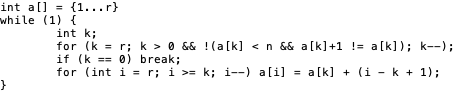
\includegraphics[scale=0.5]{a.png} \end{figure}

\fbox{\textbf{Enum r-subsets of n-set}}
\begin{figure}[h] 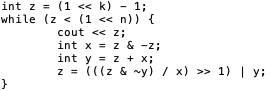
\includegraphics[scale=0.5]{b.png} \end{figure}

\noindent\rule{\linewidth}{1pt}

\fbox{\textbf{Difference table}} leftmost diagonal $= c_0, \hdots c_p, 0, \hdots $ $\rightarrow$ original sequence
\begin{align*}
	h_n &= c_0 \binom{n}{0} + \hdots + c_p \binom{n}{p} \\
	\sum_{k = 0..n}{h_k} &= c_0 \binom{n+1}{1} + \hdots + c_p \binom{n+1}{p+1}
\end{align*}

\noindent\rule{\linewidth}{1pt}

\fbox{\textbf{Catalan number}} \\ $C_n =$ \# $\pm 1$ sequences with non-negative prefix sum
\begin{align*}
	C_n &= \frac{1}{n+1} \binom{2n}{n} \\
	C_n &= \frac{4n-2}{n+1} C_{n-1}
\end{align*}

\noindent\rule{\linewidth}{1pt}

\fbox{\textbf{Stirling-1 number}} \\ $s(p,k) =$ \# $p$ diff items into $k$ same circular permutations
\begin{align*}
	s(p,0) &= 0 & (p \ge 1) \\
	s(p,p) &= 1 & (p \ge 0) \\
	s(p,k) &= (p-1) s(p-1,k) + s(p-1,k-1) & (1 \le k \le p-1) \\
	A_n^p &= \sum_{k = 0..p}{(-1)^{p-k} s(p,k) n^k}
\end{align*}

\fbox{\textbf{Stirling-2 number}} \\ $S(p,k) =$ \# $p$ diff items into $k$ same boxes, no empty box
\begin{align*}
	S(p,0) &= 0 & (p \ge 1) \\
	S(p,p) &= 1 & (p \ge 0) \\
	S(p,k) &= k S(p-1,k) + S(p-1,k-1) & (1 \le k \le p-1) \\
	S(p,k) &= \frac{1}{k!} \sum_{i = 0..k}{(-1)^i \binom{k}{i} (k-i)^p} \\
	n^p &= \sum_{k = 0..p}{S(p,k) A_n^k}
\end{align*}
\# $p$ diff items into $k$ diff boxes $= k! S(p,k)$

\fbox{\textbf{Bell number}} \\ $B_p =$ \# $p$ diff items into same boxes
\begin{align*}
	B_p &= S(p,0) + \hdots + S(p,p) \\
	B_p &= \binom{p-1}{0} B_0 + \hdots + \binom{p-1}{p-1} B_{p-1} \\
	B_{p^i+k} &\equiv i B_k + B_{k+1} \pmod{p}
\end{align*}

\noindent\rule{\linewidth}{1pt}

\fbox{\textbf{Generating function}} \\ % CF258e
$r$-combination: $\prod{(1 + x^1 + x^2 + \hdots + x^{f_i})}$ \\
$r$-arrangement: $r! \prod{(1 + \frac{x^1}{1!} + \frac{x^2}{2!} + \hdots + \frac{x^{f_i}}{f_i!})}$ \\
Integer partition: $\prod_{k = 1..n}{(1-x^k)^{-1}}$

\noindent\rule{\linewidth}{1pt}

\fbox{\textbf{Burnside lemma, Polya enum theorem}} \\
\# inequivalent colorings on $n$-set under a permutation group. 
\begin{equation*}
	N(C,G) = \frac{1}{|G|} \sum_{f \in G}{|C(f)|} = \frac{1}{|G|} \sum_{f \in G}{k^{\#(f)}} = \frac{1}{|G|} \sum_{f \in G}{k^{\sum{e_i}}}
\end{equation*}
$G$ is the equivalent permutation group \\
$C$ is all colorings on $n$-set \\
$N(C,G)$ is \# inequivalent colorings \\
$C(f)$ is the stable kernel of permutation $f$ \\
$k$ is the number of colors available \\
$\#(f)$ is the number of cycles in permutation $f$ \\
$e_1 \hdots e_n$ is the type of permutation $f$ - it has $e_i$ $i$-cycles 

\noindent\rule{\linewidth}{1pt}

\section{Graph Theory}

\fbox{\textbf{Havel-Hakimi algo}} \\ degree sequence $(d_1 \ge \hdots \ge d_n)$ is simple-graphic iff $(d_2-1 \hdots d_{d_1+1}-1, d_{d_1+2} \hdots d_n)$ is simple-graphic. Equivalently, connect largest-degree node with other largest-degree nodes. \\
Erdos-Gallai theorem: $(d_1 \ge \hdots \ge d_n)$ is simple-graphic iff
\begin{align*}
	\forall k \in [1,n] \sum_{i=1}^{k}{d_i} \le k(k-1) + \sum_{i=k+1}^{n}{\min{(d_i, k)}}
\end{align*}

\noindent\rule{\linewidth}{1pt}

\fbox{\textbf{Vizing's theorem + Misra-Gries edge coloring algo}} \\ adjacent edges cannot have same color, uses $\max{(deg(v))} + 1$ colors. 

\noindent\rule{\linewidth}{1pt}

\section{Game Theory}

\fbox{\textbf{Nim}} Lose iff XOR sum is zero

\noindent\rule{\linewidth}{1pt}

\fbox{\textbf{SG function}} \\
P-position: first lose \\
N-position: second lose \\
Final node must be P \\
N's successors contain at least one P \\
P's successors contain all N \\
$SG(x) = mex(\{SG(y) \mid \text{y is successor of x }\})$ \\
$SG(x) = 0$ iff x is P-position \\
Composite game's SG value is the XOR sum of simple games

\noindent\rule{\linewidth}{1pt}

\section{Numerical Methods}

\fbox{\textbf{Newton's method}} solve $f(x) = 0$ by $x \leftarrow x - f(x) / f'(x)$

\noindent\rule{\linewidth}{1pt}

\section{Miscellaneous}

\begin{align*}
	\gcd(2^a-1, 2^b-1) &= 2^{\gcd(a,b)}-1
\end{align*}
$x^2 + y^2 = n$ has integer solution $\leftrightarrow$ $n = \prod{p_i^{e_i}}$, there are no $i$ s.t. $p_i \equiv 3 \pmod{4}$ and $e_i \equiv 1 \pmod{2}$

\noindent\rule{\linewidth}{1pt}

\fbox{\textbf{Fibbonacci}}
\begin{align*}
	\gcd(F_n, F_m) &= F_{\gcd(n, m)} \\
	b \mid a &\leftrightarrow F_b \mid F_a
\end{align*}

\noindent\rule{\linewidth}{1pt}

\fbox{\textbf{Derangements}} \\
\begin{align*}
	D_n &= n! (1 - \frac{1}{1!} + \frac{1}{2!} - \hdots + \frac{(-1)^n}{n!}) \\
	D_n &= (n-1)(D_{n-2} + D_{n-1}) \\
	D_n &= n D_{n-1} + (-1)^n
\end{align*}

\fbox{\textbf{Gray sequence}} $G_i = i \text{ xor } (i >> 1)$

\fbox{\textbf{Farey sequence}} sorted $\frac{a}{b}$ $(1 \le a < b \le N, \gcd(a,b) = 1)$
\begin{align*}
	\frac{a_0}{b_0} &= \frac{0}{1} \\
	\frac{a_1}{b_1} &= \frac{1}{N} \\
	\frac{a_n}{b_n} &= \frac{a_{n-1} \lfloor \frac{N+b_{n-2}}{b_{n-1}} \rfloor - a_{n-2}}{b_{n-1} \lfloor \frac{N+b_{n-2}}{b_{n-1}} \rfloor - b_{n-2}}
\end{align*}

\noindent\rule{\linewidth}{1pt}

\fbox{\textbf{Dilworth theorem}} fewest chain split = longest reverse chain

\noindent\rule{\linewidth}{1pt}

\end{document}
